\documentclass[11pt]{book}
\usepackage{tikz}
\usepackage{physics}
\pgfrealjobname{myfile}
\begin{document}
\beginpgfgraphicnamed{2reflections}%
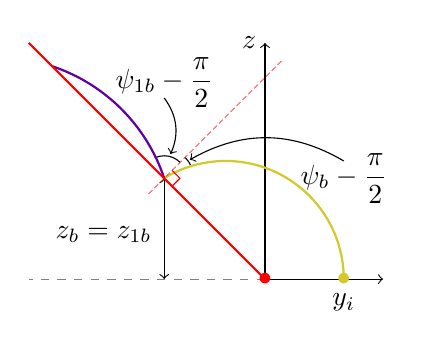
\begin{tikzpicture}[scale=1]
\draw[->] (0,0) to (0,3);


\node[] at (1,-0.3) {$y_i$};

\draw[-] (-1.28,1.28+0.286) arc (90:45:0.286);
\draw[-] (-1.28,1.28+0.286) arc (90:115:0.286);
\node at (-1.28,2.5) {$\psi_{1b}-\dfrac{\pi}{2}$};
\draw[->] (-1.28,2.3) to[bend left] (-1.2,1.28+0.306);


\draw[-] (-1.28+0.2652,1.28+0.2652) arc (45:22.5:0.375);

\node at (1,1.28) {$\psi_b - \dfrac{\pi}{2}$};
\draw[->] (1,1.5) to[bend right] (-1.28+0.3252,1.28+0.2352);


\draw[-,thick,black!20!yellow] (1,0) arc (0:180:1.5);
\draw[-,thick,purple!50!blue] (-1.28,1.28) arc (18.435:71.5653:2.25);

\draw[-,draw=none,fill=white] (-3,0) to (0,0) to (-3,3) to (-3,0);

\draw[<->] (-1.28,1.28) to (-1.28,0);
\node at (-2.05,0.57) {$z_b = z_{1b}$};

\draw[-,red,very thin,dashed,dash pattern=on 2pt off 1pt] (-1.28-0.2,1.28-0.2) to (-1.28+1.5,1.28+1.5);

\draw[-,dashed,black!50] (0,0) to (-3,0);
\draw[->] (0,0) to (1.5,0);

\node[red] at (0,0) {$\bullet$};
\node[black!20!yellow] at (1,0) {$\bullet$};

\draw[-,red,thick] (0,0) to (-3,3);


\draw[-,red] (-1.28+0.1,1.28+0.1) to (-1.28+0.2,1.28) to (-1.28+0.1,1.28-0.1);

\node at (-0.2,3) {$z$};
\end{tikzpicture}
\endpgfgraphicnamed
\end{document}